%TODO Bilder zitieren

\renewcommand{\theauthor}{Matthias Franz}
\chapter{Datenbank}
\label{sec:datenbank}
In diesem Kapitel geht es um die Datenbank welche in dieser Arbeit erstellt worden ist. Es geht um den Aufbau der Datenbank, deren Funktion und wie diese mit den anderen Teilen des Projektes zusammenarbeitet.

\section{Funktion der Datenbank}
\label{sec:funktionDatenbank}
Die Datenbank speichert Benutzerdaten und Kalender der Benutzer. Die Daten dieser Datenbank bilden alle für dieses Projekt relevanten Teile einer iCal-Datei ab. Es werden nicht alle möglichen Eigenschaften einer iCal-Datei benötigt, da die Daten welche gespeichert werden ausreichen, um einen typischen Kalender welcher in Unternehmen verwendet wird abgebildet. Die Datenbank ermöglicht es, dass mehrere Benutzer mehrere Kalender haben und mehrere Benutzer auch die gleichen Kalender haben können. Benutzer sind in der Lage Kalender mit Terminen, To-Do Elementen und Alarmen zu speichern, weiters ermöglicht die Datenbank es die Zeitzone des Kalenders zu ändern.
\\
Die Daten werden dann vom Parser genommen und in eine funktionierende .ics-Datei umgewandelt. 

\section{Aufbau der Datenbank}
\label{sec:aufbauDatenbank}
Die Datenbank ist relationale Datenbank MSSQL-Datenbank, das ER-Diagramm welches in Abbildung \ref{fig:erDiagramm} zu sehen ist wurde mit der Krähenfuß- oder auch Martinnotation abgebildet. 
\\
Ein ER-Diagramm besteht aus Entitäten und Relationen, eine Entität ist eine Tabelle und eine Relation ist eine Verbindung zweier Entitäten. Eine Relation hat immer zwei Kardinalitäten, eine Kardinalität gibt die maximal möglich Anzahl an Instanzen auf welche sich eine Entität referenzieren kann. In der Krähenfußnotation gibt es sechs verschiedene Kardinalitäten. Da auf jeder der beiden Seiten einer Relation eine Kardinalität ist, gibt es viele verschiedene Kombinationen. Alle möglichen Kardinalitäten werden in Abbildung \ref{fig:kardinalitaeten} gezeigt.
\begin{figure}[H]
	\centering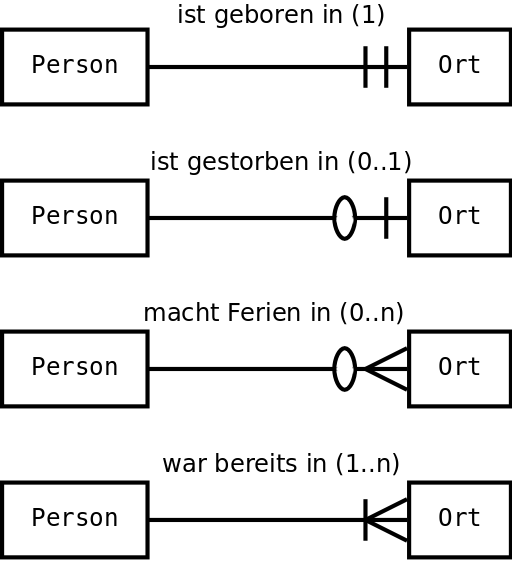
\includegraphics[scale=0.7]
	{Datenbank_Kardinalitaeten.png}
    \caption{Kardinalitäten}
    \label{fig:kardinalitaeten}
\end{figure}
Im ER-Diagramm von Abbildung \ref{fig:erDiagramm} werden Primary-Keys fett und Foreign Keys kursiv dargestellt.

\pagebreak
\begin{figure}[H]
	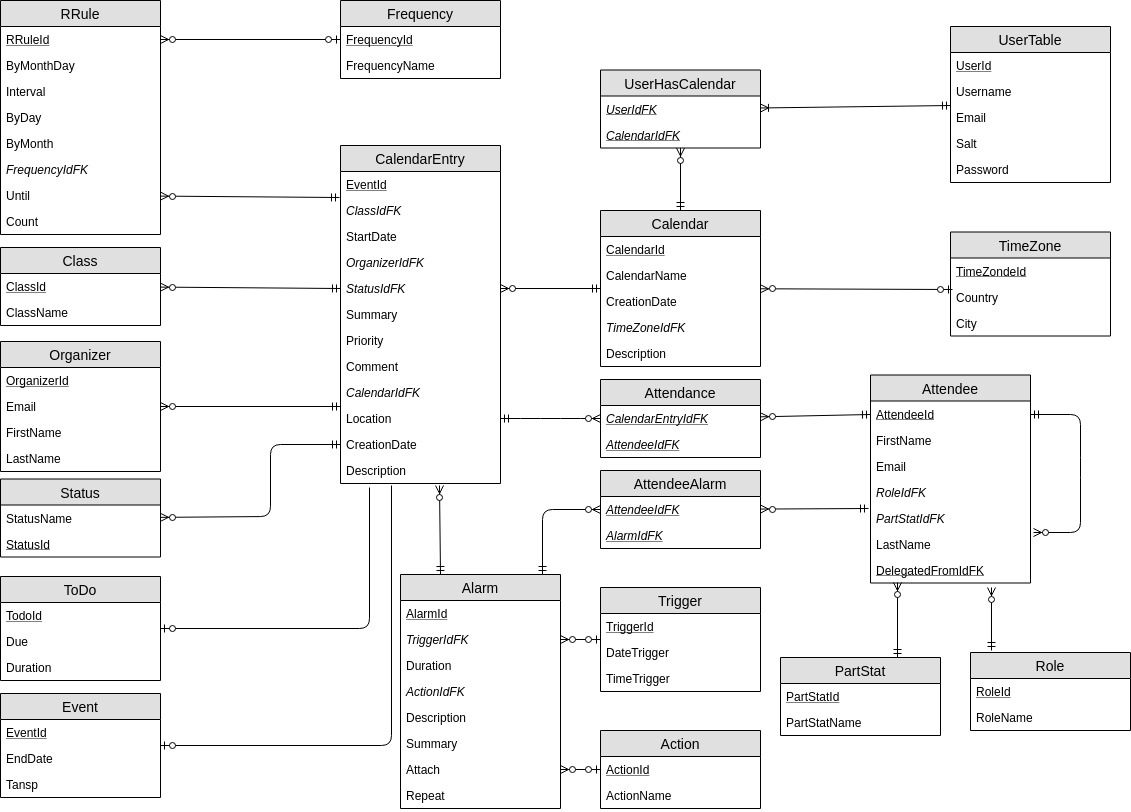
\includegraphics[angle=270,origin=c,width=\textwidth]{Datenbank_ER-Diagramm.jpg}
    \caption{ER-Diagramm}
    \label{fig:erDiagramm}
\end{figure}
	
\pagebreak